\newcommand{\svcourse}{CST Part IA: Software Engineering and Security}
\newcommand{\svnumber}{1}
\newcommand{\svvenue}{Microsoft Teams}
\newcommand{\svdate}{2022-05-11}
\newcommand{\svtime}{15:00}
\newcommand{\svuploadkey}{CBd13xmL7PC1zqhNIoLdTiYUBnxZhzRAtJxv/ytRdM1r7qIfwMsxeVwM/pPcIo8l}

\newcommand{\svrname}{Dr Sam Ainsworth}
\newcommand{\jkfside}{oneside}
\newcommand{\jkfhanded}{yes}

\newcommand{\studentname}{Harry Langford}
\newcommand{\studentemail}{hjel2@cam.ac.uk}


\documentclass[10pt,\jkfside,a4paper]{article}

% DO NOT add \usepackage commands here.  Place any custom commands
% into your SV work files.  Anything in the template directory is
% likely to be overwritten!

\usepackage{fancyhdr}

\usepackage{lastpage}       % ``n of m'' page numbering
\usepackage{lscape}         % Makes landscape easier

\usepackage{verbatim}       % Verbatim blocks
\usepackage{listings}       % Source code listings
\usepackage{graphicx}
\usepackage{float}
\usepackage{epsfig}         % Embed encapsulated postscript
\usepackage{array}          % Array environment
\usepackage{qrcode}         % QR codes
\usepackage{enumitem}       % Required by Tom Johnson's exam question header

\usepackage{hhline}         % Horizontal lines in tables
\usepackage{siunitx}        % Correct spacing of units
\usepackage{amsmath}        % American Mathematical Society
\usepackage{amssymb}        % Maths symbols
\usepackage{amsthm}         % Theorems

\usepackage{ifthen}         % Conditional processing in tex

\usepackage[top=3cm,
            bottom=3cm,
            inner=2cm,
            outer=5cm]{geometry}

% PDF metadata + URL formatting
\usepackage[
            pdfauthor={\studentname},
            pdftitle={\svcourse, SV \svnumber},
            pdfsubject={},
            pdfkeywords={9d2547b00aba40b58fa0378774f72ee6},
            pdfproducer={},
            pdfcreator={},
            hidelinks]{hyperref}

\renewcommand{\headrulewidth}{0.4pt}
\renewcommand{\footrulewidth}{0.4pt}
\fancyheadoffset[LO,LE,RO,RE]{0pt}
\fancyfootoffset[LO,LE,RO,RE]{0pt}
\pagestyle{fancy}
\fancyhead{}
\fancyhead[LO,RE]{{\bfseries \studentname}\\\studentemail}
\fancyhead[RO,LE]{{\bfseries \svcourse, SV~\svnumber}\\\svdate\ \svtime, \svvenue}
\fancyfoot{}
\fancyfoot[LO,RE]{For: \svrname}
\fancyfoot[RO,LE]{\today\hspace{1cm}\thepage\ / \pageref{LastPage}}
\fancyfoot[C]{\qrcode[height=0.8cm]{\svuploadkey}}
\setlength{\headheight}{22.55pt}


\ifthenelse{\equal{\jkfside}{oneside}}{

 \ifthenelse{\equal{\jkfhanded}{left}}{
  % 1. Left-handed marker, one-sided printing or e-marking, use oneside and...
  \evensidemargin=\oddsidemargin
  \oddsidemargin=73pt
  \setlength{\marginparwidth}{111pt}
  \setlength{\marginparsep}{-\marginparsep}
  \addtolength{\marginparsep}{-\textwidth}
  \addtolength{\marginparsep}{-\marginparwidth}
 }{
  % 2. Right-handed marker, one-sided printing or e-marking, use oneside.
  \setlength{\marginparwidth}{111pt}
 }

}{
 % 3. Alternating margins, two-sided printing, use twoside.
}


\setlength{\parindent}{0em}
\addtolength{\parskip}{1ex}

% Exam question headings, labels and sensible layout (courtesy of Tom Johnson)
\setlist{parsep=\parskip, listparindent=\parindent}
\newcommand{\examhead}[3]{\section{#1 Paper #2 Question #3}}
\newenvironment{examquestion}[3]{
\examhead{#1}{#2}{#3}\setlist[enumerate, 1]{label=(\alph*)}\setlist[enumerate, 2]{label=(\roman*)}
\marginpar{\href{https://www.cl.cam.ac.uk/teaching/exams/pastpapers/y#1p#2q#3.pdf}{\qrcode{https://www.cl.cam.ac.uk/teaching/exams/pastpapers/y#1p#2q#3.pdf}}}
\marginpar{\footnotesize \href{https://www.cl.cam.ac.uk/teaching/exams/pastpapers/y#1p#2q#3.pdf}{https://www.cl.cam.ac.uk/\\teaching/exams/pastpapers/\\y#1p#2q#3.pdf}}
}{}


\usepackage{dirtytalk}

\begin{document}

\part{Worksheet 2}

\section{Natural Languages}

\begin{enumerate}

\item Write a paragraph on the following open-ended point to discuss with
your supervisor

\begin{itemize}

\item[-] Is frequency information or structural information more important
when considering processing difficulty?

\end{itemize}

I consider structural information to be more important when considering
processing difficulty. While the probabilities of words are relevant, there
are simply structures which are challenging to parse. I give an example from
Shakespeare's Macbeth:

\begin{center}
\begin{minipage}{0.6\textwidth}
Doubtful it stood;\\
As two spent swimmers, that do cling together\\
And choke their art. The merciless Macdonwald--\\
Worthy to be a rebel, for to that\\
The multiplying villanies of nature\\
Do swarm upon him--from the western isles\\
Of kerns and gallowglasses is supplied;\\
And fortune, on his damned quarrel smiling,\\
Show'd like a rebel's whore: but all's too weak:\\
For brave Macbeth--well he deserves that name--\\
Disdaining fortune, with his brandish'd steel,\\
Which smoked with bloody execution,\\
Like valour's minion carved out his passage\\
Till he faced the slave;\\
Which ne'er shook hands, nor bade farewell to him,\\
Till he unseam'd him from the nave to the chaps,\\
And fix'd his head upon our battlements.
\end{minipage}
\end{center}

This quote describes a brutal battle with ``brave Macbeth'' slaying the
rebel Macdonwald. However, it's almost impossible to read. All the
sentences are individually comprehensible; however once they're combined into
one long sentence, they're impossible to parse. The words which Shakespeare
uses are used on modern English; all with moderately high probability.
However, the sentence structures which he use are outdated and not found in
modern English. This makes any extended sentences impossible to parse. If
these sentences were restructured to use modern English structures, we would
be able to parse them far easier. I believe there is \textit{no assignment of
words} such that a sentence with the same structure as this quote from
Macbeth would be easily understandable to a normal English speaker. While
there are many sentence structures such that the same words could be used
to convey Shakespeare's original meaning:
\begin{center}
\begin{minipage}{0.6\textwidth}
It stood doubtful; like two spent swimmers clinging together and choking
each other.
\end{minipage}
\end{center}

\item Give examples and counter-examples of sentences in English (or any
other language) that would support theories of constant information rate
(try to think of examples that are different from those provided in the slides!)

Consider the following passage:
\begin{center}
\begin{minipage}{0.6\textwidth}
The quality of programmers is a decreasing function of the density of
\textbf{go to} statements in their programs. I recently discovered the
disastrous effects the \textbf{go to} statement has, and became convinced
the \textbf{go to} statement should be abolished from all ``higher level''
languages. I did not attach importance to this; I submit considerations for
publication because when the subject turned up I was urged to do so.
\end{minipage}
\end{center}

Now consider the original passage from Edskar Dijkstra's ``Go To Statement
Considerd Harmful'':
\begin{center}
\begin{minipage}{0.6\textwidth}
For  number of years I have been familiar with the observation that the
quality of programmers is a decreasing function of the density of
\textbf{go to} statements in the programs they produce. More recently I
discovered why the use of the \textbf{go to} statement has such disastrous
effects, and I became convinced that the \textbf{go to} statement should be
abolished from all ``higher level'' programming languages (i.e. everything
except, perhaps, plain machine code). At that time I did not attach too much
importance to this discovery; I now submit my considerations for publication
because in very recent discussions in which the subject turned up, I have
been urged to do so.
\end{minipage}
\end{center}

Throughout this quote, Edgskar is discussing a topic which (at the time) was
not commonly discussed. Furthermore, this is an introduction and so people
have little contextual information about which to decrease the information
rate. Therefore, the entropy of every sentence is high. As such, in the
original quote, connectives are introduced at every opportunity to decrease
the entropy rate as far as possible. The modified version removed all
connectives to increase the entropy rate and as such is harder to parse.

\end{enumerate}

\section{Formal Languages and Learnability}

\begin{enumerate}

\item Consider a rigid classic categorial grammar $C_{cg} = (\Sigma, P_r, S,
\mathcal R)$ where $P_r = \{S, X\}$, $\Sigma = \{a, b, c, d, e\}$ and $S =
S$. If $a$, $b$ have type $X$ and you know that $abc \in \mathcal L(C_{c})$,
$abdc \in \mathcal L(C_{cg})$, $ebc \in \mathcal L(C_{cg})$, give possible
types for each of $c$, $d$ and $e$?

\[
\{(c, X \setminus X \setminus S), (d, X \setminus X), (e, X)\}
\]

\item Explain why a finite class of finite languages is learnable within
Gold's paradigm.

Under Golds paradigm, if the language which we are recognising is finite
then the learner will be fed exhaustive data -- every sample in the data.
It's therefore trivial to build a learning function $\mathcal F$ which
output the language containing the set $S$ of strings $s$ which
$\mathcal F$ has been fed.

\item Describe a learning paradigm where a learner could learn from two
sources simultaneously (bilingual)

Define a grammatical system $(\mathcal H, \Omega, \mathcal L)$ as follows:
\begin{itemize}

\item $\mathcal H$ is the hypothesis space -- the set of all pairs of
languages $(L_1, L_2)$ of the form
$((\mathcal N_1, \Sigma_1, \mathcal P_1, S_1),
(\mathcal N_2, \Sigma_2, \mathcal P_2, S_2))$ where $\mathcal P$ is
restricted to allow only grammars below a certain complexity.

\item $\Omega$ is the set of strings which are visible. For example, the set
$(\Sigma_1^*, \Sigma_2^*)$.

\item $\mathcal L$ is a function from $\mathcal H \to \Omega$ which
specifies the set of languages which each of the grammars can generate.

\end{itemize}

The learning paradigm is then specified as follows:

\begin{itemize}

\item A pair $(L_1, L_2) \in \mathcal L$ is selected as the target language

\item All samples $(s_1, s_2)$ are taken from the hypothesis space $\Omega$

\item The learner receives samples $(s_1, s_2)$ from the learner in an
infinite sequence.

\item After receiving each sample, the learner produces a hypothesis
$(G_{i_1}, G_{i_2}) \in \mathcal G$.

\item Learning is successful when $(G_1, G_2)$ have both been identified in
the limit.

\end{itemize}

\end{enumerate}

\section{Information Theory}

\begin{enumerate}

\item A binary symmetric channel is one where the input $x_i$ and the output
$y_i$ are both in $\{0, 1\}$. The channel is characterised by $p$ the
probability that an input bit is transmitted as the opposite bit. If $q$ is
the probability that the source sends $x = 0$, and $1 - q$ the probability
of $x = 1$, show tht the mutual information is maximised when zeros and ones
are transmitted with equal probability (i.e when $q = 0.5$).

Using the definition for mutual information and distributivity of partial
differentiation over addition:
\begin{align*}
I(X_i; Y_i)
&= H(Y_i) - H(Y_i|X_i) \\
\frac{\partial I(X_i; Y_i)}{\partial q}
&= \frac{\partial H(Y_i)}{\partial q} - \frac{\partial H(Y_i|X_i)}{\partial
q} \\
\end{align*}
I will now consider each case separately:
\begin{align*}
H(Y_i)
&= -\sum_{y_i \in \{0, 1\}} p(y_i) \lg p(y_i) \\
&= - (pq + (1-p)(1-q)) \lg (pq + (1-p)(1-q)) - (p(1-q) + (1-p)q)\lg(p(1-q) + (1-p)q) \\
&= - (1 - p - q + 2pq) \lg (1 - p - q + 2pq) - (p + q - 2pq)\lg(p + q - 2pq) \\
\frac{\partial H(Y_i)}{\partial q}
&= -(2p - 1)\lg (1 - p - q + 2pq) - (2p - 1) + (2p - 1)\lg(p + q - 2pq) +
(2p - 1) \\
&= (2p - 1)\lg \frac{p + q - 2pq}{1 - p - q + 2pq}
\\\\
H(Y_i|X_i)
&=
-\sum_{x_i \in \{0, 1\}}
\sum_{y_i \in \{0, 1\}}
p(x_i, y_i)\lg p(y_i|x_i) \\
&= - p(1-q) \lg p - pq\lg p - (1-p)q\lg (1-p) - (1-p)(1-q)\lg (1-p) \\
\frac{\partial H(Y_i|X_i)}{\partial q}
&= p\lg p - p\lg p - (1-p)\lg(1-p) + (1-p)\lg(1-p) \\
&= 0
\end{align*}
Substituting into the original formula gives:
\begin{align*}
\frac{\partial I(X_i|Y_i)}{\partial q}
&=
(2p - 1)\lg \frac{p + q - 2pq}{1 - p - q + 2pq} \\
0 &=
(2p - 1)\lg \frac{p + q - 2pq}{1 - p - q + 2pq} \\
0 &=
\lg \frac{p + q - 2pq}{1 - p - q + 2pq} \\
1 &= \frac{p + q - 2pq}{1 - p - q + 2pq} \\
1 - p - q + 2pq &= p + q - 2pq \\
0 &= 4pq - 2p - 2q + 1 \\
0 &= (2p - 1)(2q - 1) \\
0 &= 2q - 1 \\
q &= \frac{1}{2}
\end{align*}

\item Using the processed Alice in Wonderland file write some simple code to
generate some good candidates for nonsense words by:

\begin{itemize}[label = -]

\item finding the probability distribution defined by a bigram langauge model

\item generating some words using the probability distribution

\item selecting the 10 words whose information rate is lowest

\end{itemize}

\begin{table}[H]
\centering
\begin{tabular}{c|c}
word & information rate \\
\hline
a & 0.023684605006745612 \\
i & 0.01536501274171789 \\
ani & 0.007926312071608285 \\
thchi & 0.007209095652393102 \\
thi & 0.004004583532064527 \\
ini & 0.0031108113059844437 \\
ali & 0.002623860223613271 \\
wii & 0.002328867707379849 \\
ati & 0.0018429980959495836 \\
bei & 0.0017422835462293014
\end{tabular}
\end{table}


\item Describe how you could frame the following tasks as noisy channel
problems:

\begin{itemize}[label = -]

\item automatically answering questions

We could consider the following framework:

\begin{figure}[H]
\centering
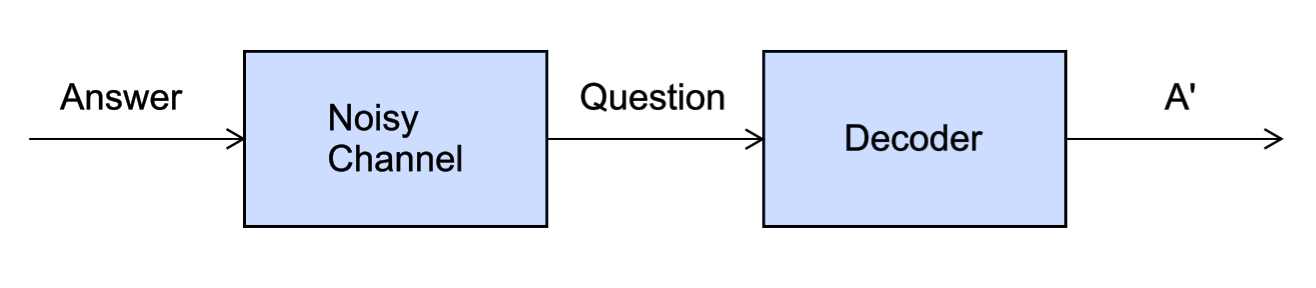
\includegraphics[width=0.6\textwidth]{noisychannel}
\end{figure}

In this framework, we phrase the problem of answering a question as ``the
answer which is most likely to have caused the user to answer the question''.
This allows us to use Bayes' Rule -- since $P(Q|A)$ is likely easier to
compute than $P(A|Q)$. For example, this problem would become trivial if we
restricted the format of answers to yes/no and modelled questions as a
bi-gram model while the other direction would remain almost intractable.

\item disambiguating multiple senses of a word

Consider the following framework:

\begin{figure}[H]
\centering
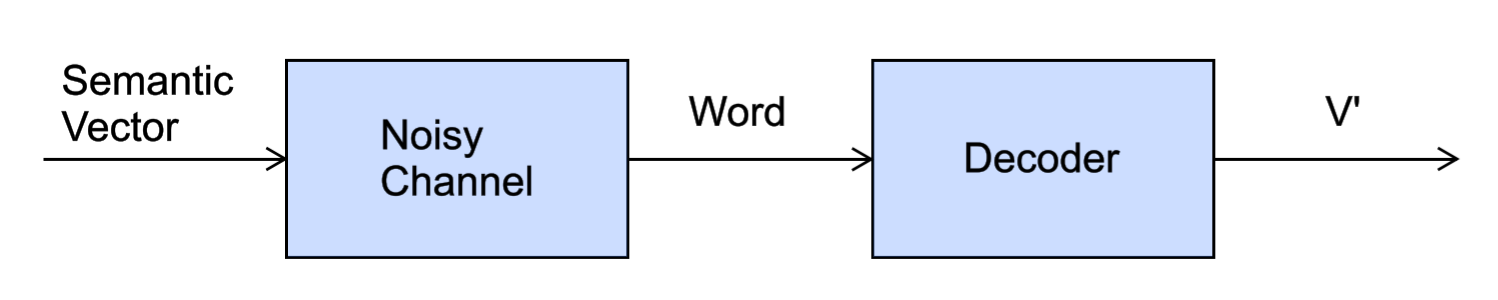
\includegraphics[width=0.6\textwidth]{meaningchannel}
\end{figure}

We represent this problem as ``trying to establish the semantic meaning of a
word from the word presented''. Phrasing this as ``establishing the vector
which was most likely to have generated that word'' is far easier than
directly approaching the reverse direction.

\end{itemize}

\end{enumerate}

\section{Distributional Models}

\begin{enumerate}

\item Describe how you might use word distributions to compare the
similarity of two characters in a text. What might any \textit{similarity}
be telling us about the characters.

I would build a vector representation of each of the characters -- the
simplest approach would use a count model, although a predict model would
yield better results. I would then consider the unit vector in the direction
of the representation of the characters.

An even better approach to building a vector representation would use an
approach similar to that taken by a GNN\@. Consider each word to be a node
and let there be an edge $u \to v$ if word $u$ occurs close to word $v$ with
the weight of the edge as the number of co-occurrences of $v$ near $u$ divided
by the total number words which occur near $u$. Then let the vector
representation of a node be an aggregation of the count model representation
of all adjacent nodes (possibly after some dimensionality reduction i.e from
the encoder of an encoder-decoder architecture).

\end{enumerate}

\begin{examquestion}{2022}{7}{5}

\textbf{Most of this was done under exam conditions and in exam time}.
Part of (b) is in italics -- this was done when typesetting the question.
Apologies for the strange typesetting of probabilities. That was done in
exam time.

\begin{enumerate}

\item You have the following sentences translated from English into Triposi.

\begin{table}[H]
\centering
\begin{tabular}{l|l}
English & Triposi \\
\hline
she drinks water
&
mwamni sileg \\
the rain soaks the teacher
&
sileng mworob sesesrakan \\
the teacher drinks here
&
sesesrakan mwamni mwabma \\
the teacher keeps drinking
&
sesesrakan mwatbo mwamni
\end{tabular}
\end{table}

\begin{enumerate}

\item Translate the following English sentences into Triposi:\\
\textit{the rain keeps soaking the teacher}\\
\textit{she keeps drinking water here}

sileng mworob mwabma sesesrakan

mwatbo mwamni mwamba

\item Describe how we can calculate the likelihood of a translation using
the noisy channel framework: you will need to give and explain the equation
for decoding from one language into another, and explain how you can obtain
the information needed to carry out the calculations.

The noisy channel framework is as follows:
Input $X$ sent across a noisy channel as form $Y$ (with some probability of
corruption). The receiver then receives $Y$ and has to estimate $X'$ --
the $X$ with maximal probability of having generated $Y$.

We can use this to translate from one language to another using the
following framework:

English -> Triposi -> English'

So we try to find the English sentence which was most likely to have
generated the Triposi sentence.

Firstly, we design a model and then fit it using a corpus of training data
(or prior knowledge about the triposi grammar).

We then take a data-science approach by using Bayes rule to find a maximum
apriori estimator for English' given the Triposi.

\[
English' = \text{argmax}_{English} P(English|Triposi)
= \text{argmax}_{English} \frac{P(Triposi|English)P(English)}{P(Triposi)}
\]
We can find this either by numerical optimisation (gradient search or a
known formula) or mathematically by differentiation.

\item What problem do the following underlined English words present, given
the training data we have so far, and how can you still translate them into
Triposi with a machine? \textit{the \underline{teachers} drink
\underline{Perrier}}

The underlined English words are not present in the training corpus. This
means distributional models will be unable to even represent their existence
-- let alone translate them! And any model taking a learning approach will
not have a means of translation.

We could use a distributional semantics to build a predict language model,
which represents each word in a vector space. Then, we could replace the
absent words with their closest English word for which we have a
translation. This would largely preserve meaning -- although not entirely.
The likely translation would be ``the teacher drinks water'' which captures
some but not all of the essence of the sentence.

\end{enumerate}

\item You know that your optical character recognition model has made errors
on every predicted instance of `e'. Explain what information you need in
order to automatically correct these errors with a noisy channel approach.

We need to know (or have an estimate of) the \textit{probability} of
different types of errors occurring -- the probability of ``e'' being
mistranslated to any other letter. The noisy channel approach attempts
to discover $X' \text{argmax}_{X} P(X|Y)$ -- its not possible to do this without
knowing what the error rate of the channel is.

\textit{Furthermore we must also know the prior probability of the letter `e'
being sent across the channel. A good model would take this probability
given the context (i.e using a 2nd order model), however any model would be
sufficient. Bayes rule needs priors to work.}

\[
English' = \text{argmax}_{English} P(English|Triposi)
= \text{argmax}_{English} \frac{P(Triposi|English)P(English)}{P(Triposi)}
\]

\item A signaller sends you Morse code messages, but you know that they send
a dot when they should send a dash two times in five, and a dash instead of
a dot three times in ten. You also know that they use the character M $(--)$
3 times in 100, N $(-\cdot)$ and I $(\cdot\cdot)$ 7/100 and A
$(\cdot-)$ 8/100.

You receive the message ``$\cdot\cdot\ -\cdot\ \cdot-$''. What is the
likelihood that it represents MIN, MAN, NAN or AIM?

Note that I use likelihoods -- the actual probability depends on the
probability of the message being sent at all -- for which we have
insufficient information.

The probability of a dash transitioning to a dot is 0.4

The probability of a dot transitioning to a dash os 0.3

The probability of M is 0.03

The probability of N is 0.07

The probability of I is 0.07

The probability of A is 0.08

We can use Bayes rule to work out the probability.

MIN is (-- .. -.) The probability of MIN|.. -. .- is

\[
\frac{P(Message|Min)P(Min)}{P(M)}
= \kappa P(Message|Min)P(Min)
= \kappa (0.4 * 0.4 * 0.3 * 0.7 * 0.4 * 0.3) * (0.03 * 0.07 * 0.07)
\]

MAN is (-- .. -.) The probability of MAN|.. -. .- is

\[
\frac{P(Message|Man)P(Man)}{P(M)}
= \kappa P(Message|Man)P(Man)
= \kappa (0.4 * 0.4 * 0.3 * 0.4 * 0.4 * 0.3) * (0.03 * 0.08 * 0.07)
\]

NAN is (-- .. -.) The probability of NAN|.. -. .- is

\[
\frac{P(Message|Nan)P(Nan)}{P(M)}
= \kappa P(Message|Nan)P(Nan)
= \kappa (0.4 * 0.7 * 0.3 * 0.4 * 0.4 * 0.3) * (0.07 * 0.08 * 0.07)
\]

AIM is (-- .. -.) The probability of AIM|.. -. .- is

\[
\frac{P(Message|Aim)P(Aim)}{P(M)}
= \kappa P(Message|Aim)P(Aim)
= \kappa (0.7 * 0.4 * 0.3 * 0.7 * 0.4 * 0.6) * (0.08 * 0.07 * 0.03)
\]

\item Discuss the similarities and differences between the noisy channel and
human processing of spoken English.

The noisy channel model (which we have discussed) is a 1st order model.
Human processing of spoken English is certainly a 2nd order model -- one
which takes the full context into account (this greatly decreases ambiguity).

The noisy channel model only takes sentence units into account -- spoken
English contains extra information such as prosidy (intonation, tone) or
disfluency / false starts (which indicate a topic is more challenging).

Furthermore, there is evidence that humans slow their speaking to make the
information rate uniform.

The noisy channel model also assumes perfect knowledge -- humans do not have
perfect knowledge. When we encounter a person for the first time (or a
person initiates a conversation) we often struggle to understand them. I
believe this is because our priors for what this person may be saying are
not set. We therefore expect them to say something totally different. The
noisy channel framework would be unable to deal with a situation such as
this (or otherwise have an overly simplistic model).

\end{enumerate}

\end{examquestion}

\end{document}
